\section{. Mathematical Analysis of a Secretion Model}
\label{appendix:Analysis}

\cite{siguenza2017Ae4} constructed a single salivary gland acinar cell secretion model with the purpose of supporting and explaining experimental results in which mouse submandibular salivary glands exhibit a decrease in fluid flow rate upon anion exchanger \textit{Slc4a9} (Ae4) knockout \citep{pena2015ae4}. The study addressed a long standing hypothesis concerning the involvement of the anion exchanger \textit{Slc4a2} (Ae2) in the fluid secretion process \citep{evans2000severe}. The model's results indicate that the cation-dependence of the Ae4 is favourable for water transport in acinar cells, as opposed to the Ae2. Although we can observe that an Ae4 knockout has different effects in secretion than does an Ae2 knockout, and we can hypothesise that this difference is due to cation transport, our understanding of this difference remains limited and hampered due to excessive model complexity.\\

In an attempt to resolve this problem, here we determine the simplest possible model in which this same phenomenon occurs. We then show that, in this simple model, the inclusion of $\na$ transport is sufficient to explain the observed differences between Ae4 and Ae2 knockout experiments.

\subsection{Simple Model $\&$ Non-dimensionalisation}
%The model presented in \cite{siguenza2017Ae4} has two physiologically relevant steady states. The first of these represents the cellular resting state (or basal secretory state). Here,  as $\cl$ and $\kplus$ enter the cytoplasm, $\na$ is actively extruded against its concentration gradient. The energy generated by this exchange is used by the PM machinery to concentrate $\cl$ further, well above its electrochemical gradient. What drives the change from the resting state to a stimulated salivation steady state is a change in the $\bc$, a parameter of the model. An increase in $\bc$ initiates the extrusion of $\cl$ towards the acinar lumen whilst $\kplus$ is released towards the interstitium. The transcellular movement of $\cl$ creates an osmotic gradient which water follows by osmosis. The model's results show that the fluid flow rate of the cell at rest in the Ae4 knockout case is the same as the control (or when there is no knockout). However, when stimulation occurs (by increasing $\bc$ from 0.058$\mu$M to 0.25$\mu$M) there is a considerable decrease in fluid flow rate compared to the control. In contrast, the Ae2 knockout results demonstrate that absence of the mechanism does not affect the transport of water in the cell at rest or under stimulation.\\

\subsubsection*{Simple Model}
As we seek a simple model detailing the relationship between $\na$ and the basic secretion mechanism described above, we focus only on the dynamics of $\bna$, $\bkplus$, and $\bcl$. The rest of the intracellular ionic concentrations are assumed constant. The assumption stems from the fact that in \cite{siguenza2017Ae4}, the [H$^+$]$_i$ and $\bcot$ are practically constant at rest and stimulation. However $\bhco$ is not, but the intracellular pH has been experimentally observed to remain relatively constant at rest and salivation in acinar cells \citep{pena2015ae4}.  \\

We assume the ionic concentrations in the lumen constant as these vary very little from rest to secretion \citep{siguenza2017Ae4}.  The apical PM has a relatively high permeability to water (proportional to the density of aquaporins), and as a result the osmotic gradient between the cell and the lumen must not be too big in order for a relatively substantial amount of fluid to be transported. The constant approximation allows us to ignore the dynamics of the lumen and concentrate on the intracellular concentrations and the PM mechanisms of the cell  \citep{maclaren2012efficiency}.\\

Additionally, the PM membrane potentials ($V_a$ and $V_b$) are also assumed constant. In the basic secretory mechanism, activation of the $\cl$ and $\kplus$ channels must happen nearly simultaneously. As a result, the transcellular PM potential is kept virtually constant at -60 mV \citep{nauntofte1992regulation}.\\

We define the apical secretion rate by using a convection equation for steady state one dimensional flow \citep{kedem1958thermodynamic}:
\begin{align}
\label{eq:appendix_Q}
& q_a=  L_a V_w \Bigg( 2 ( [\na]_l + [\kplus]_l ) + \Psi_l - 2 ( \bna + \bkplus + [\text{H}^+]_i) + \bcot \Bigg),
\end{align}
where the parameter $L_a$ is the apical PM permeability (proportional to the density of aquaporins) with units of $\mu$m$^3$/sec, and $V_w$ the molality of water with units of mM$^{-1}$. The parameter $\Psi_l$ represents the concentration uncharged molecules in the lumen that contribute to the osmolarity of the compartment that we do not account for (with units of mM$^{-1}$). See table~\ref{table:Par} for a description of the parameters and their values. Note that $\bcl$ and $\bhco$ do not appear in the equation describing the cellular fluid flow rate. This is a consequence of the electroneutrality constraint in the cell (for more details see \cite{siguenza2017Ae4}). \\
 
The simplified system of equations is given by:
\begin{align*}
&  \frac{d\Big(\omega{_i} \bna\Big)}{dt}=J_{\text{Nkcc1}}-3J_{\text{NaK}}+J_{\text{Nhe1}}-J_{\text{Ae4}},\\
&  \frac{d\Big(\omega{_i}\bkplus\Big)}{dt}=J_{\text{Nkcc1}}+2J_{\text{NaK}}-J_{\text{K}}, \\
&  \frac{d\Big(\omega{_i} \bcl\Big)}{dt}=2J_{\text{Nkcc1}}+J_{\text{Ae4}}+J_{\text{Ae2}}-J_{\text{Cl}}.
\end{align*}
A full description of the fluxes can be found in \citep{siguenza2017Ae4}. As a final assumption we let the cellular volume $\omega_i$ to be constant. The assumption, although incorrect, allows for the simplification of the secretion model without having to account for a fourth differential equation, and thus reducing the complexity of the analysis.\\

%

%The respective concentration values were chosen according to the steady state given when $\bc = 0.25$ $\mu$M. In \cite{siguenza2017Ae4} $\bc$ is a parameter that drives transcellular movement of $\cl$ and therefore secretion in the model. This precise value represents the stimulated secretion steady state (by cholinergic agonists). We focus on the steady sate given by this value, as it is where the effects of the Ae2 and Ae4 knockouts are observable (\citealt{pena2015ae4}; \citealt{siguenza2017Ae4}). The latter allows to keep the cellular volume ($\omega_i$) constant. Consequently, we can write a simplified system consisting of the following 3 differential equations:



%The simplified system allows us to focus on the basic interplay between the three ions in the cell and their role in water transport across the cell whilst omitting the complicated dynamics of pH regulation and luminal concentrations. Let:
\subsubsection*{Non-dimensionalisation}

As we are concerned with the qualitative behaviour of the model, we seek a non-dimensional system of equations that reproduce the model's results. In this light, we define the following scaled variables:

\begin{align*}
& x = \frac{q_{a_0}}{G_1} \bna,\\
& y = \frac{q_{a_0}}{G_1} \bkplus,\\
& z = \frac{q_{a_0}}{G_1} \bcl,\\
& \tau = \frac{t}{T}.
\end{align*}
Accordingly $\tau$, $x$, $y$, and $z$ are the scaled time ($t$), $\bna$, $\bkplus$, and $\bcl$, respectively. Here we have chosen $G_1$, the activity parameter of the Nhe1 antiporter, with units of $\text{amol}/\text{seconds}$, and the basal fluid flow rate $q_{a_0}$ with units of $\mu m^3/ \text{seconds}$, as scaling parameters (see Table~\ref{table:Par}). $T$ is also a scaling parameter for time ($t$), with units of seconds. Then,
\begin{align}
& \frac{dx}{d\tau}=j_{\text{Nkcc1}}-3j_{\text{NaK}}+ j_{\text{Nhe1}}-j_{\text{Ae4}},\\
&\frac{dy}{d\tau}=j_{\text{Nkcc1}}+2 j_{\text{NaK}}-j_{\text{K}},\\
& \frac{dz}{d\tau}=2j_{\text{Nkcc1}}+j_{\text{Ae4}}+j_{\text{Ae2}}-j_{\text{Cl}}.
\end{align}
where the notation $j$ denotes the non-dimensional fluxes. The non-dimensional $ j_{\text{Ae2}}$ and $j_{\text{Ae4}}$ are defined as follows: 
{\small
\begin{align*}
&j_{\text{Ae2}} = G_{2}\left(\lambda_{17}-\frac{\lambda_{18}z}{z+\lambda_{19}}\right),
\end{align*}
}
{\small
\begin{align*}
&  j_{\text{Ae4}}= G_{4}\left( \lambda_{11}x-\lambda_{12}z\right).
\end{align*}
}
Where $G_2$ and $G_4$ are the densities of the transporters (see table~\ref{table:lambda}). The non-dimensional water flow rate is given by:
{\small
\begin{align}
\label{eq:non_Q}
Q=\Bigg(\frac{L_a V_w G_1}{q_{a_0}^2}\Bigg) \Bigg( 2 ( x_l + y_l ) + \Psi_l - 2 ( x + y + h_i) + co_2 \Bigg) = \lambda_{20}-\lambda_{21} \Bigg( x + y \Bigg),
\end{align}
}
We have used the notation, $\lambda_i$, $i=1,...,21$ to simplify the simplified parameters of the model according to the flux terms described in \cite{siguenza2017Ae4}. Their values can be found in table~\ref{appendix:parameters}.\\
\begin{table}
\centering
\captionsetup{justification=centering} 
\caption{Parameters of the model.}
\begin{adjustbox}{max width=1.0\textwidth}
\begin{tabular}{@{}llll@{}}
\toprule 
\bf{Parameter}	& \bf{Value}	 	&\bf{Parameter} 			& \bf{Value}		\\ \midrule
$\lambda_1$		& 16.266			& $\lambda_{14}$			& 71.750	 		\\ 
$\lambda_2$		& 2074819.479	& $\lambda_{15}$			& 191.363		\\
$\lambda_3$ 		& 1.03			& $\lambda_{16}$			& 56.925	 		\\
$\lambda_4$ 		& 1385200		& $\lambda_{17}$			& 20.421			\\
$\lambda_5$ 		& 38.545			& $\lambda_{18}$			& 16.179			\\	
$\lambda_6$ 		& 0.00002809		& $\lambda_{19}$ 		& 5.6			\\	
$\lambda_7$		& 0.641			& $\lambda_{20}$			& 0.472			\\
$\lambda_8$		& 8.466			& $\lambda_{21}$			& 0.003			\\
$\lambda_9$		& 3.473			& $G_{4}$	& 6.74e-5		\\		
$\lambda_{10}$	& 15	 			& $G_{2}$	& 0.347			\\
$\lambda_{11}$ 	& 4589.648		& $x_0$ 					& 12.29	 		\\
$\lambda_{12}$	& 13.423			& $y_0$ 					& 89.19			\\
$\lambda_{13}$	& -313.123		& $z_0$ 					& 37.13			\\ 										
\bottomrule
\end{tabular}
\end{adjustbox}
\label{table:lambda}
\end{table}

Finally, we are interested in the relationship between the Ae4 flux term and $\bna$ with respect to the secretion rate of the system, given by eq.~(\ref{eq:non_Q}). As the distinction between Ae4/Ae2 knockouts and control fluid flow rates are evident during the secretion steady state (or when $\bc = 0.25 \mu$M), we focus only on the steady state corresponding to the stimulated secretion \citep{siguenza2017Ae4}. Assuming this steady state, we perform one last simplification: 
\begin{align}
\label{eq:f1}
& j_{\text{Nkcc1}}-3j_{\text{NaK}}+ j_{\text{Nhe1}}-j_{\text{Ae4}} =0,\\
\label{eq:f2}
&j_{\text{Nkcc1}}+2 j_{\text{NaK}}-j_{\text{K}} =0,\\
\label{eq:f3}
& 3j_{\text{Nkcc1}}-3j_{\text{NaK}}+j_{\text{Nhe1}}+j_{\text{Ae2}}-j_{\text{Cl}}=0.
\end{align} 
Here, we have simplified the system such that eq.~\eqref{eq:f1} contains the only Ae4 flux term in the system. Similarly, eq.~\eqref{eq:f3} is the only term containing the Ae2 flux ($j_{\text{Ae2}}$). For simplicity we denote eqs.~(\ref{eq:f1} - \ref{eq:f3}), as $f_1$, $f_2$, and $f_3$, respectively. 
\subsection{Analysis}
%%%%%%%%%%%%%%%%%%%%%%%%%%%
\begin{figure}
\centering
\captionsetup[subfigure]{justification=centering, labelfont={bf}}
      \begin{subfigure}{0.49\textwidth}
               \caption{\hspace*{\fill}}
               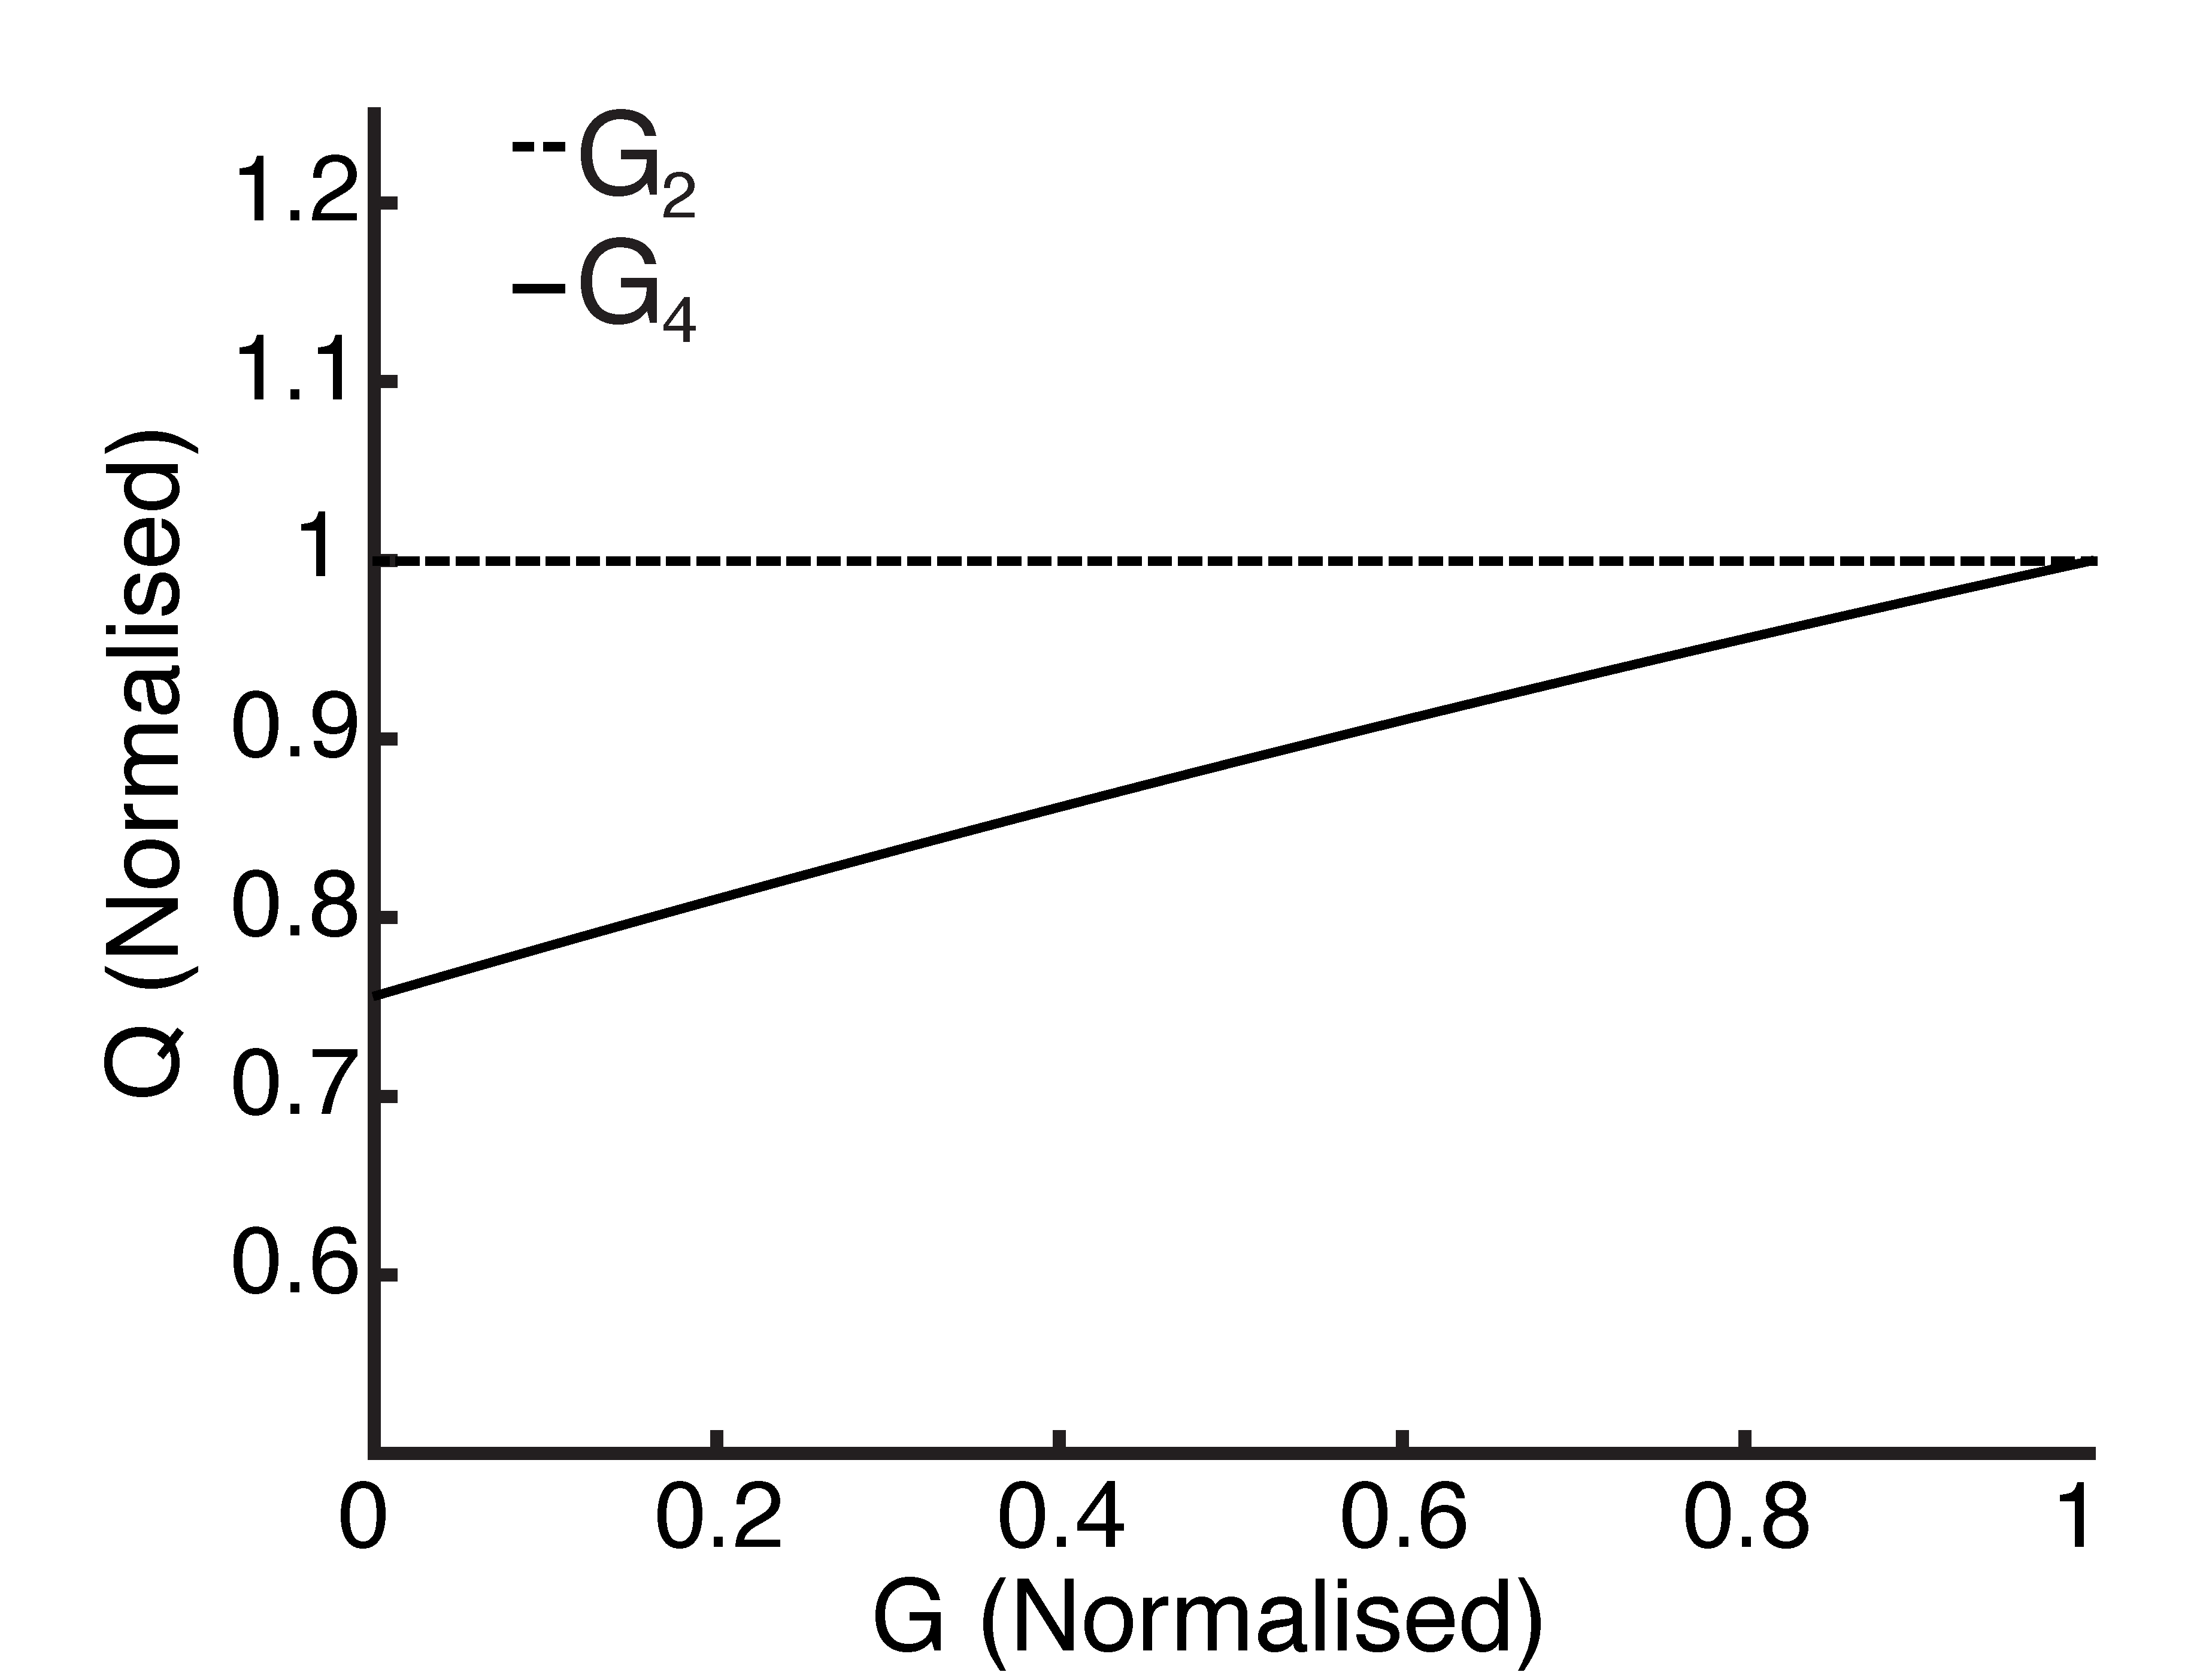
\includegraphics[width=\linewidth]{Figure3.pdf}
               \label{fig:}
       \end{subfigure}
      \begin{subfigure}{0.49\textwidth}
               \caption{\hspace*{\fill}}
               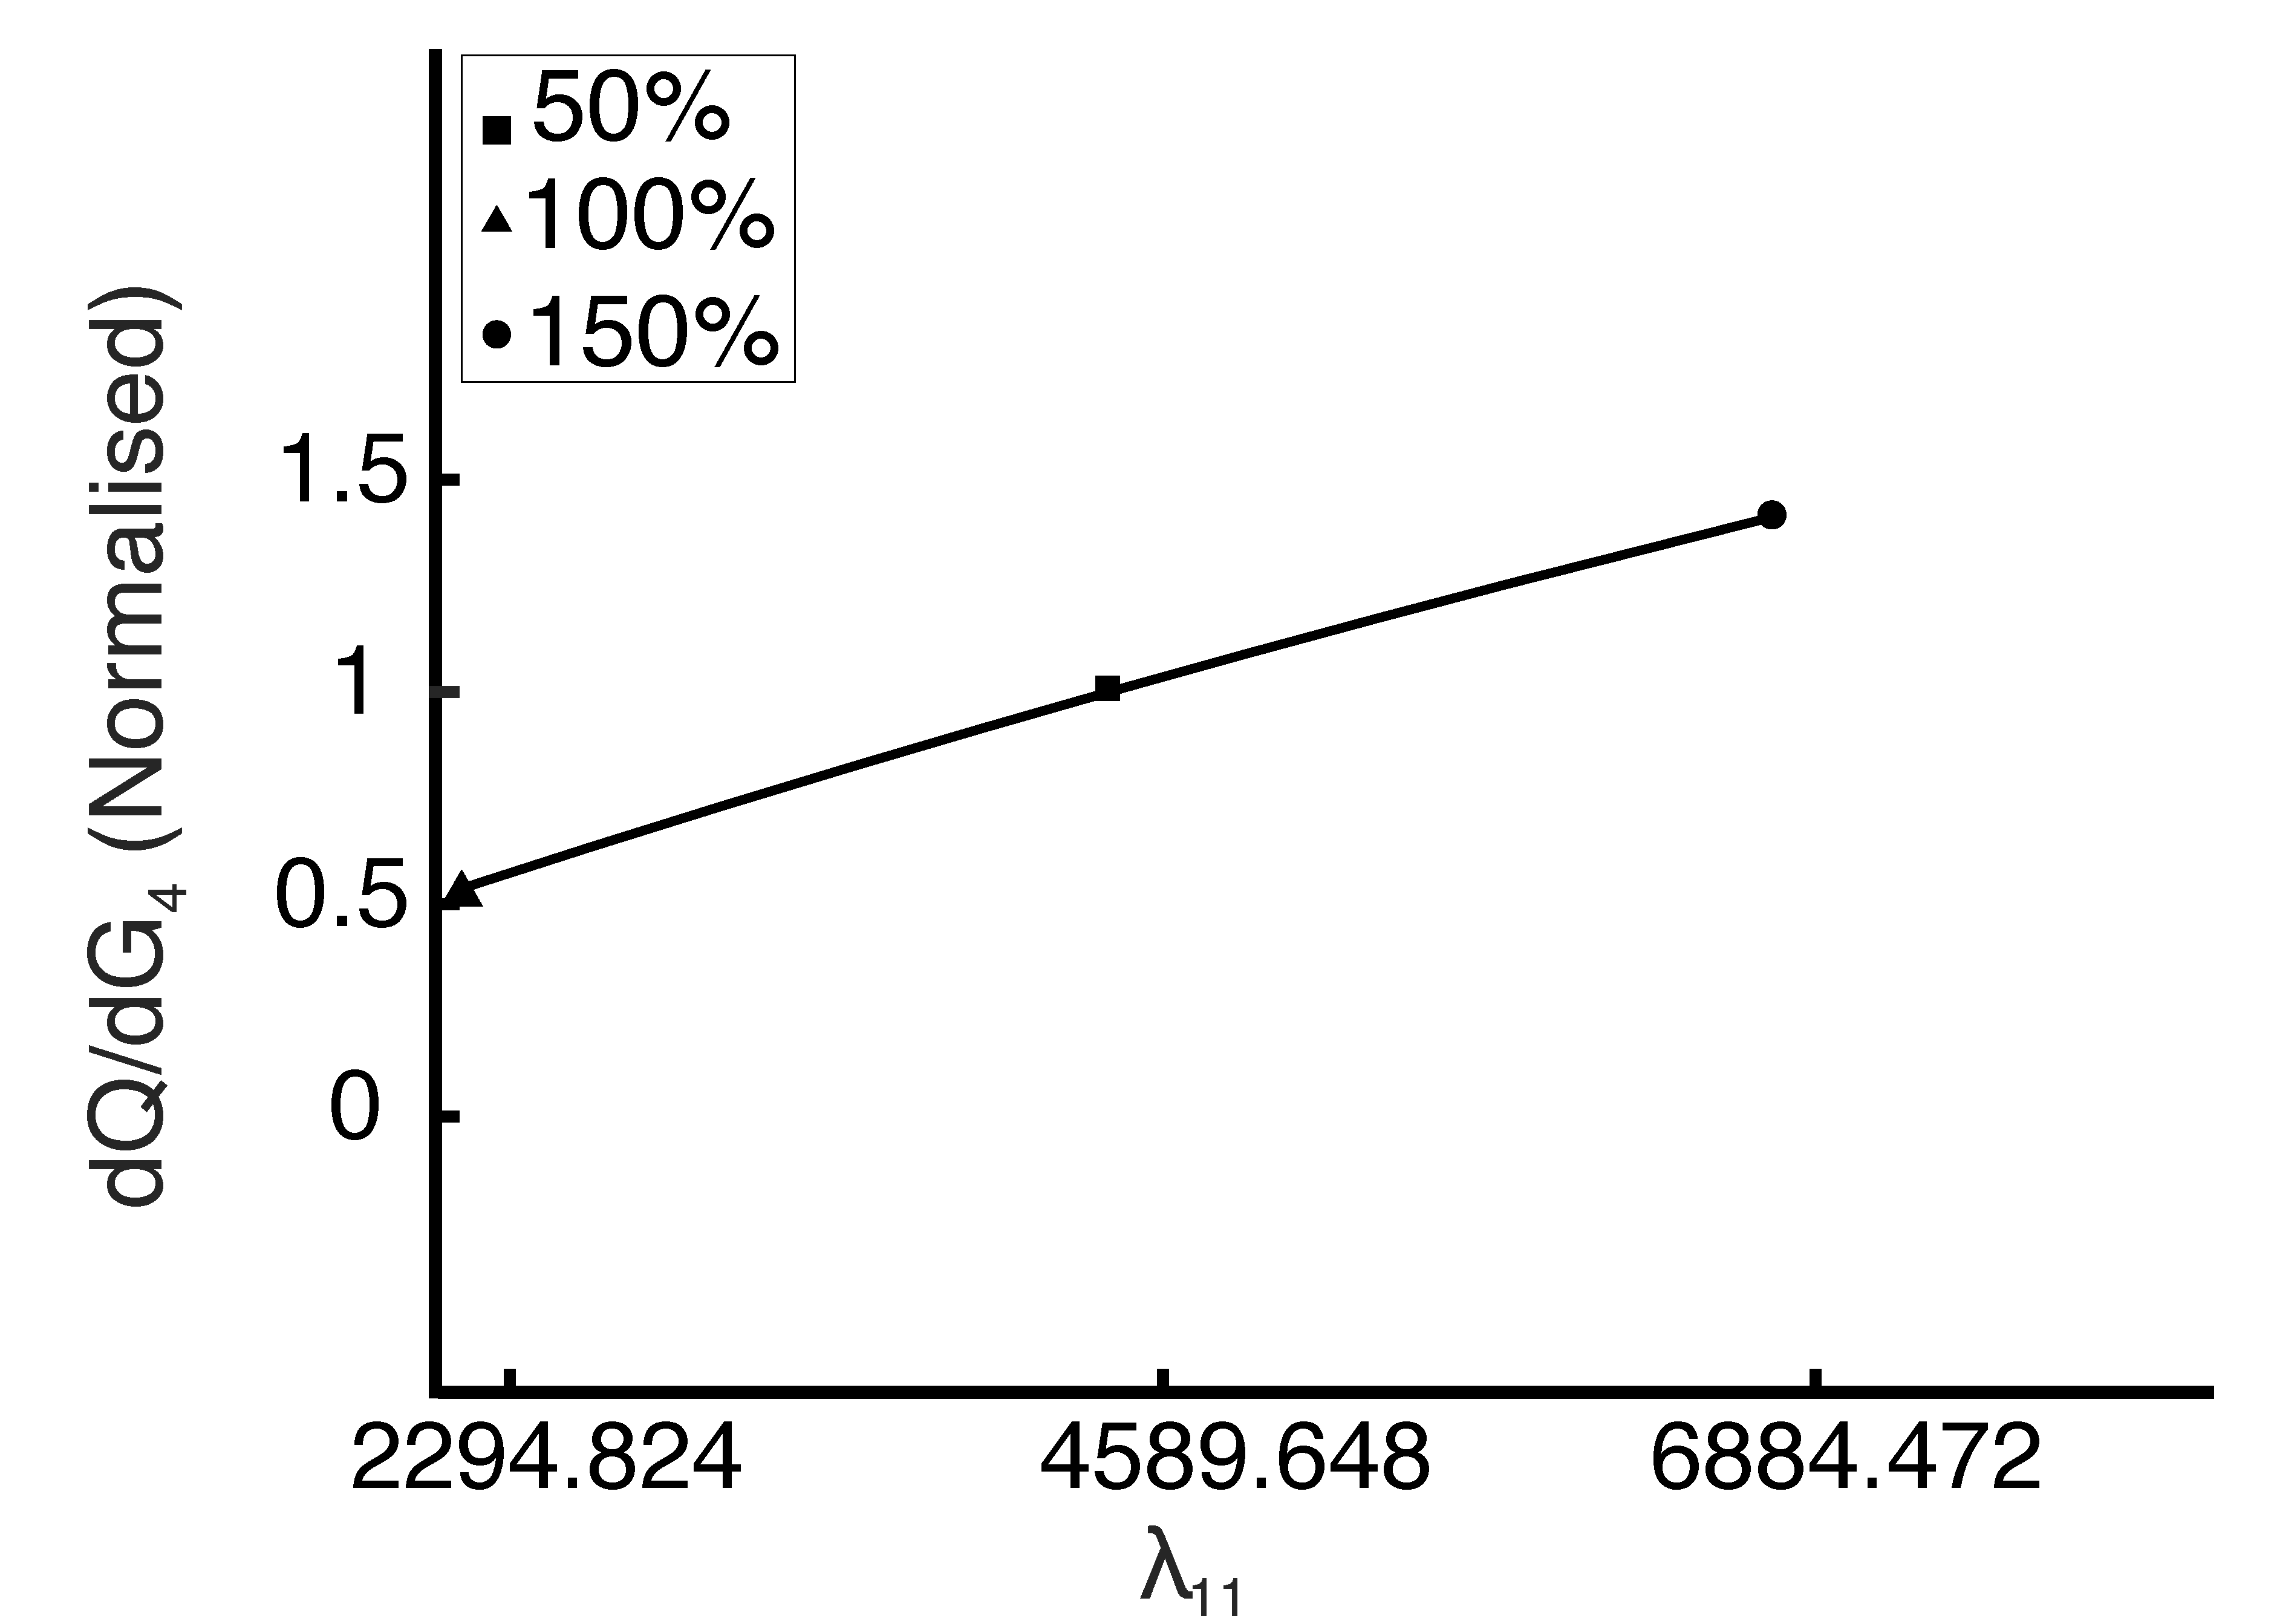
\includegraphics[width=\linewidth]{Figure8.pdf}
               \label{fig:}
       \end{subfigure}


        \begin{subfigure}{0.49\textwidth}
               \caption{\hspace*{\fill}}
               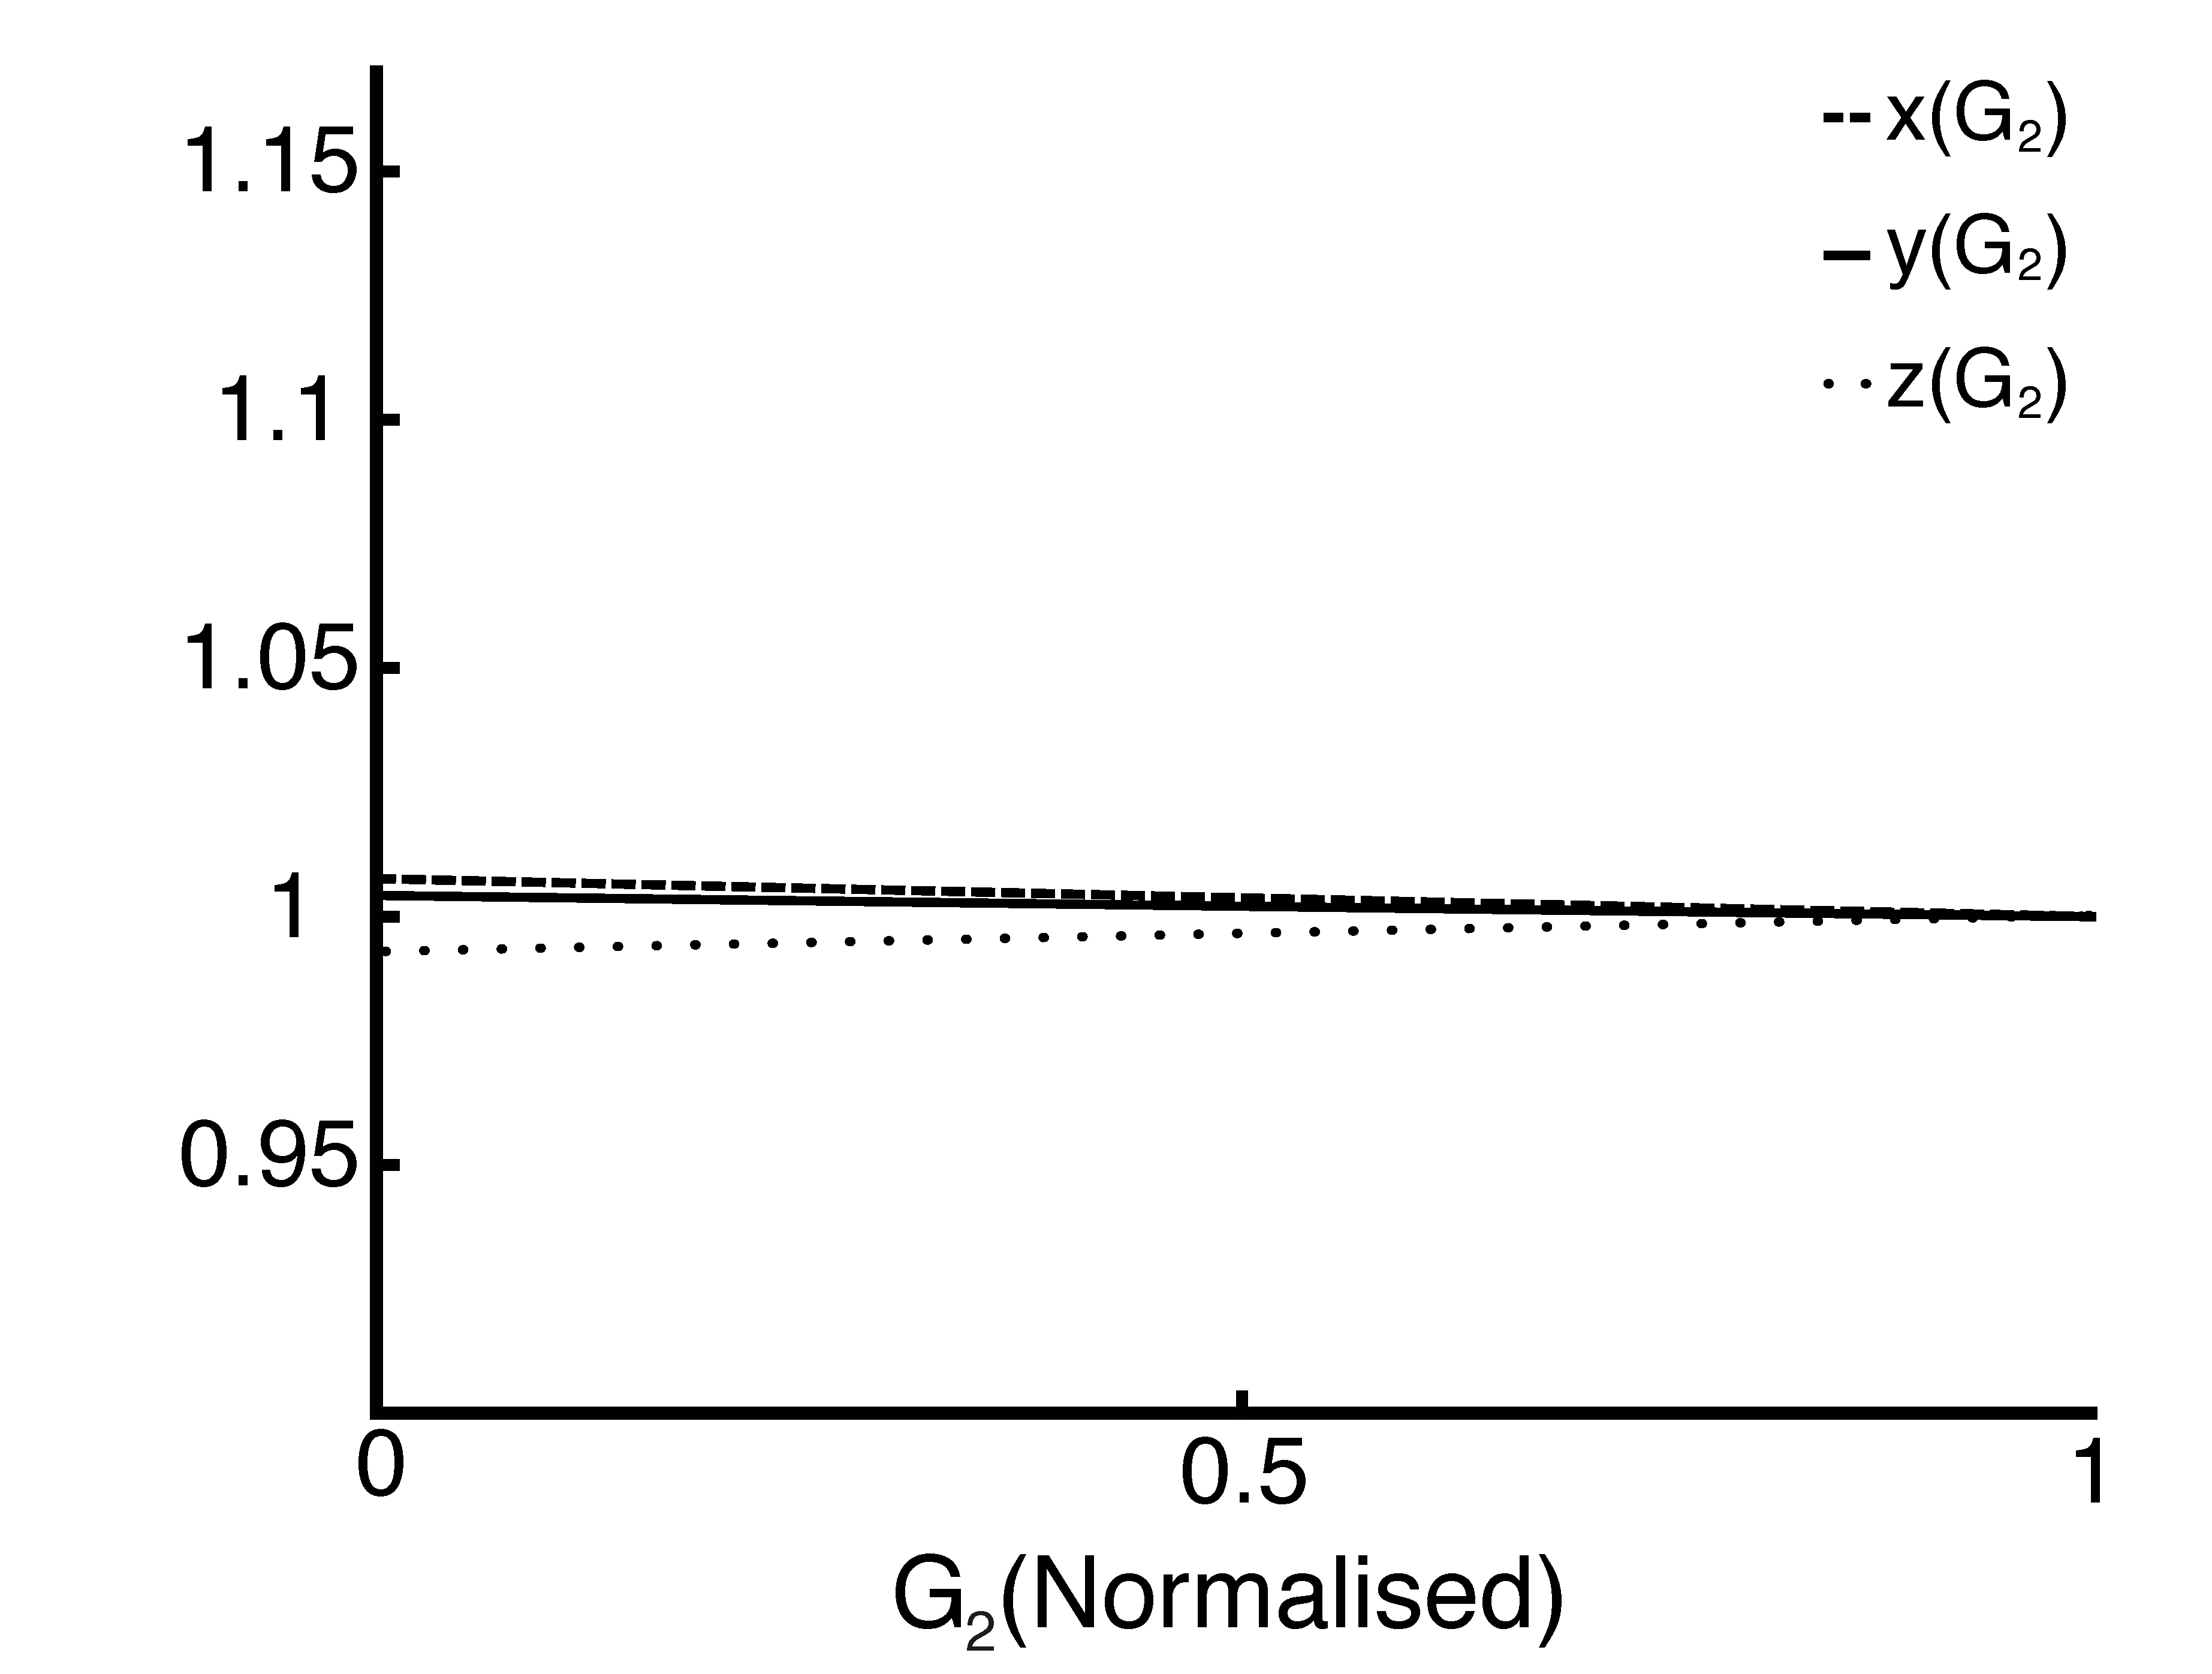
\includegraphics[width=\linewidth]{Figure7.pdf}
               \label{fig:}
       \end{subfigure}
  		 \begin{subfigure}{0.49\textwidth}
               \caption{\hspace*{\fill}}
               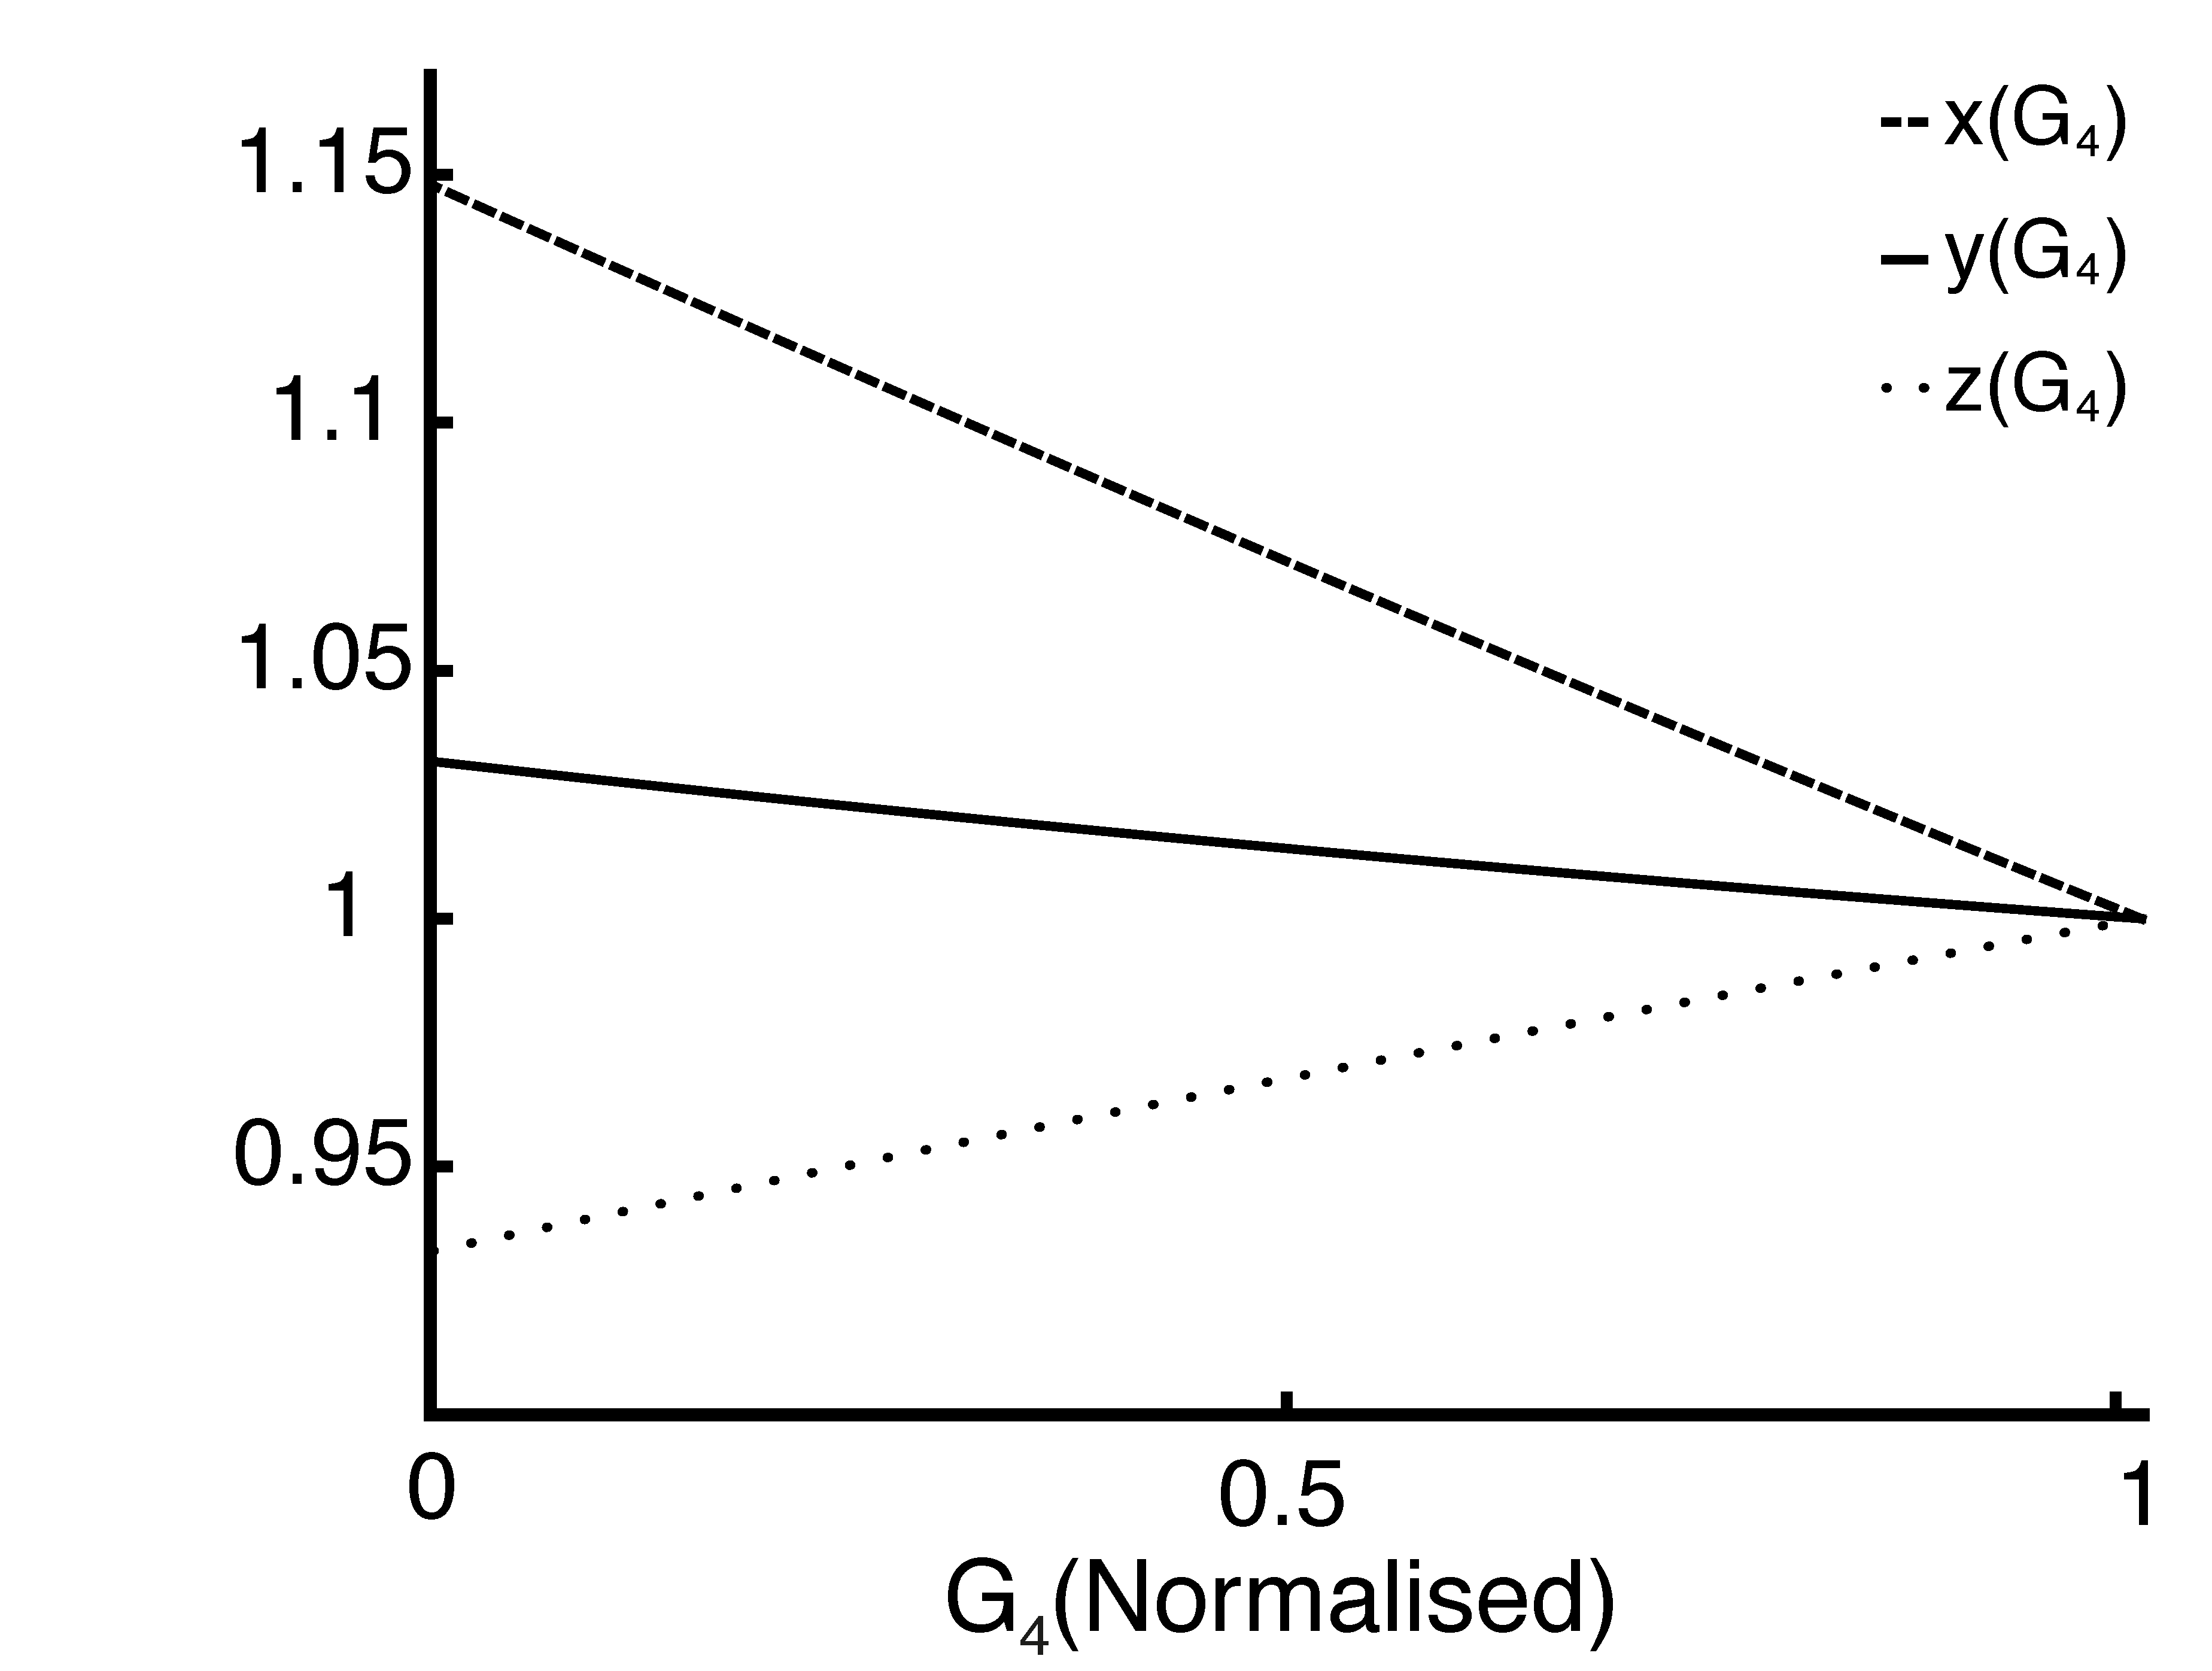
\includegraphics[width=\linewidth]{Figure6.pdf}
               \label{fig:}
       \end{subfigure}
\end{figure}
\begin{figure}
\centering
\captionsetup[subfigure]{justification=centering, labelfont={bf}}
       \begin{subfigure}{0.49\textwidth}
               \caption{\hspace*{\fill}}
               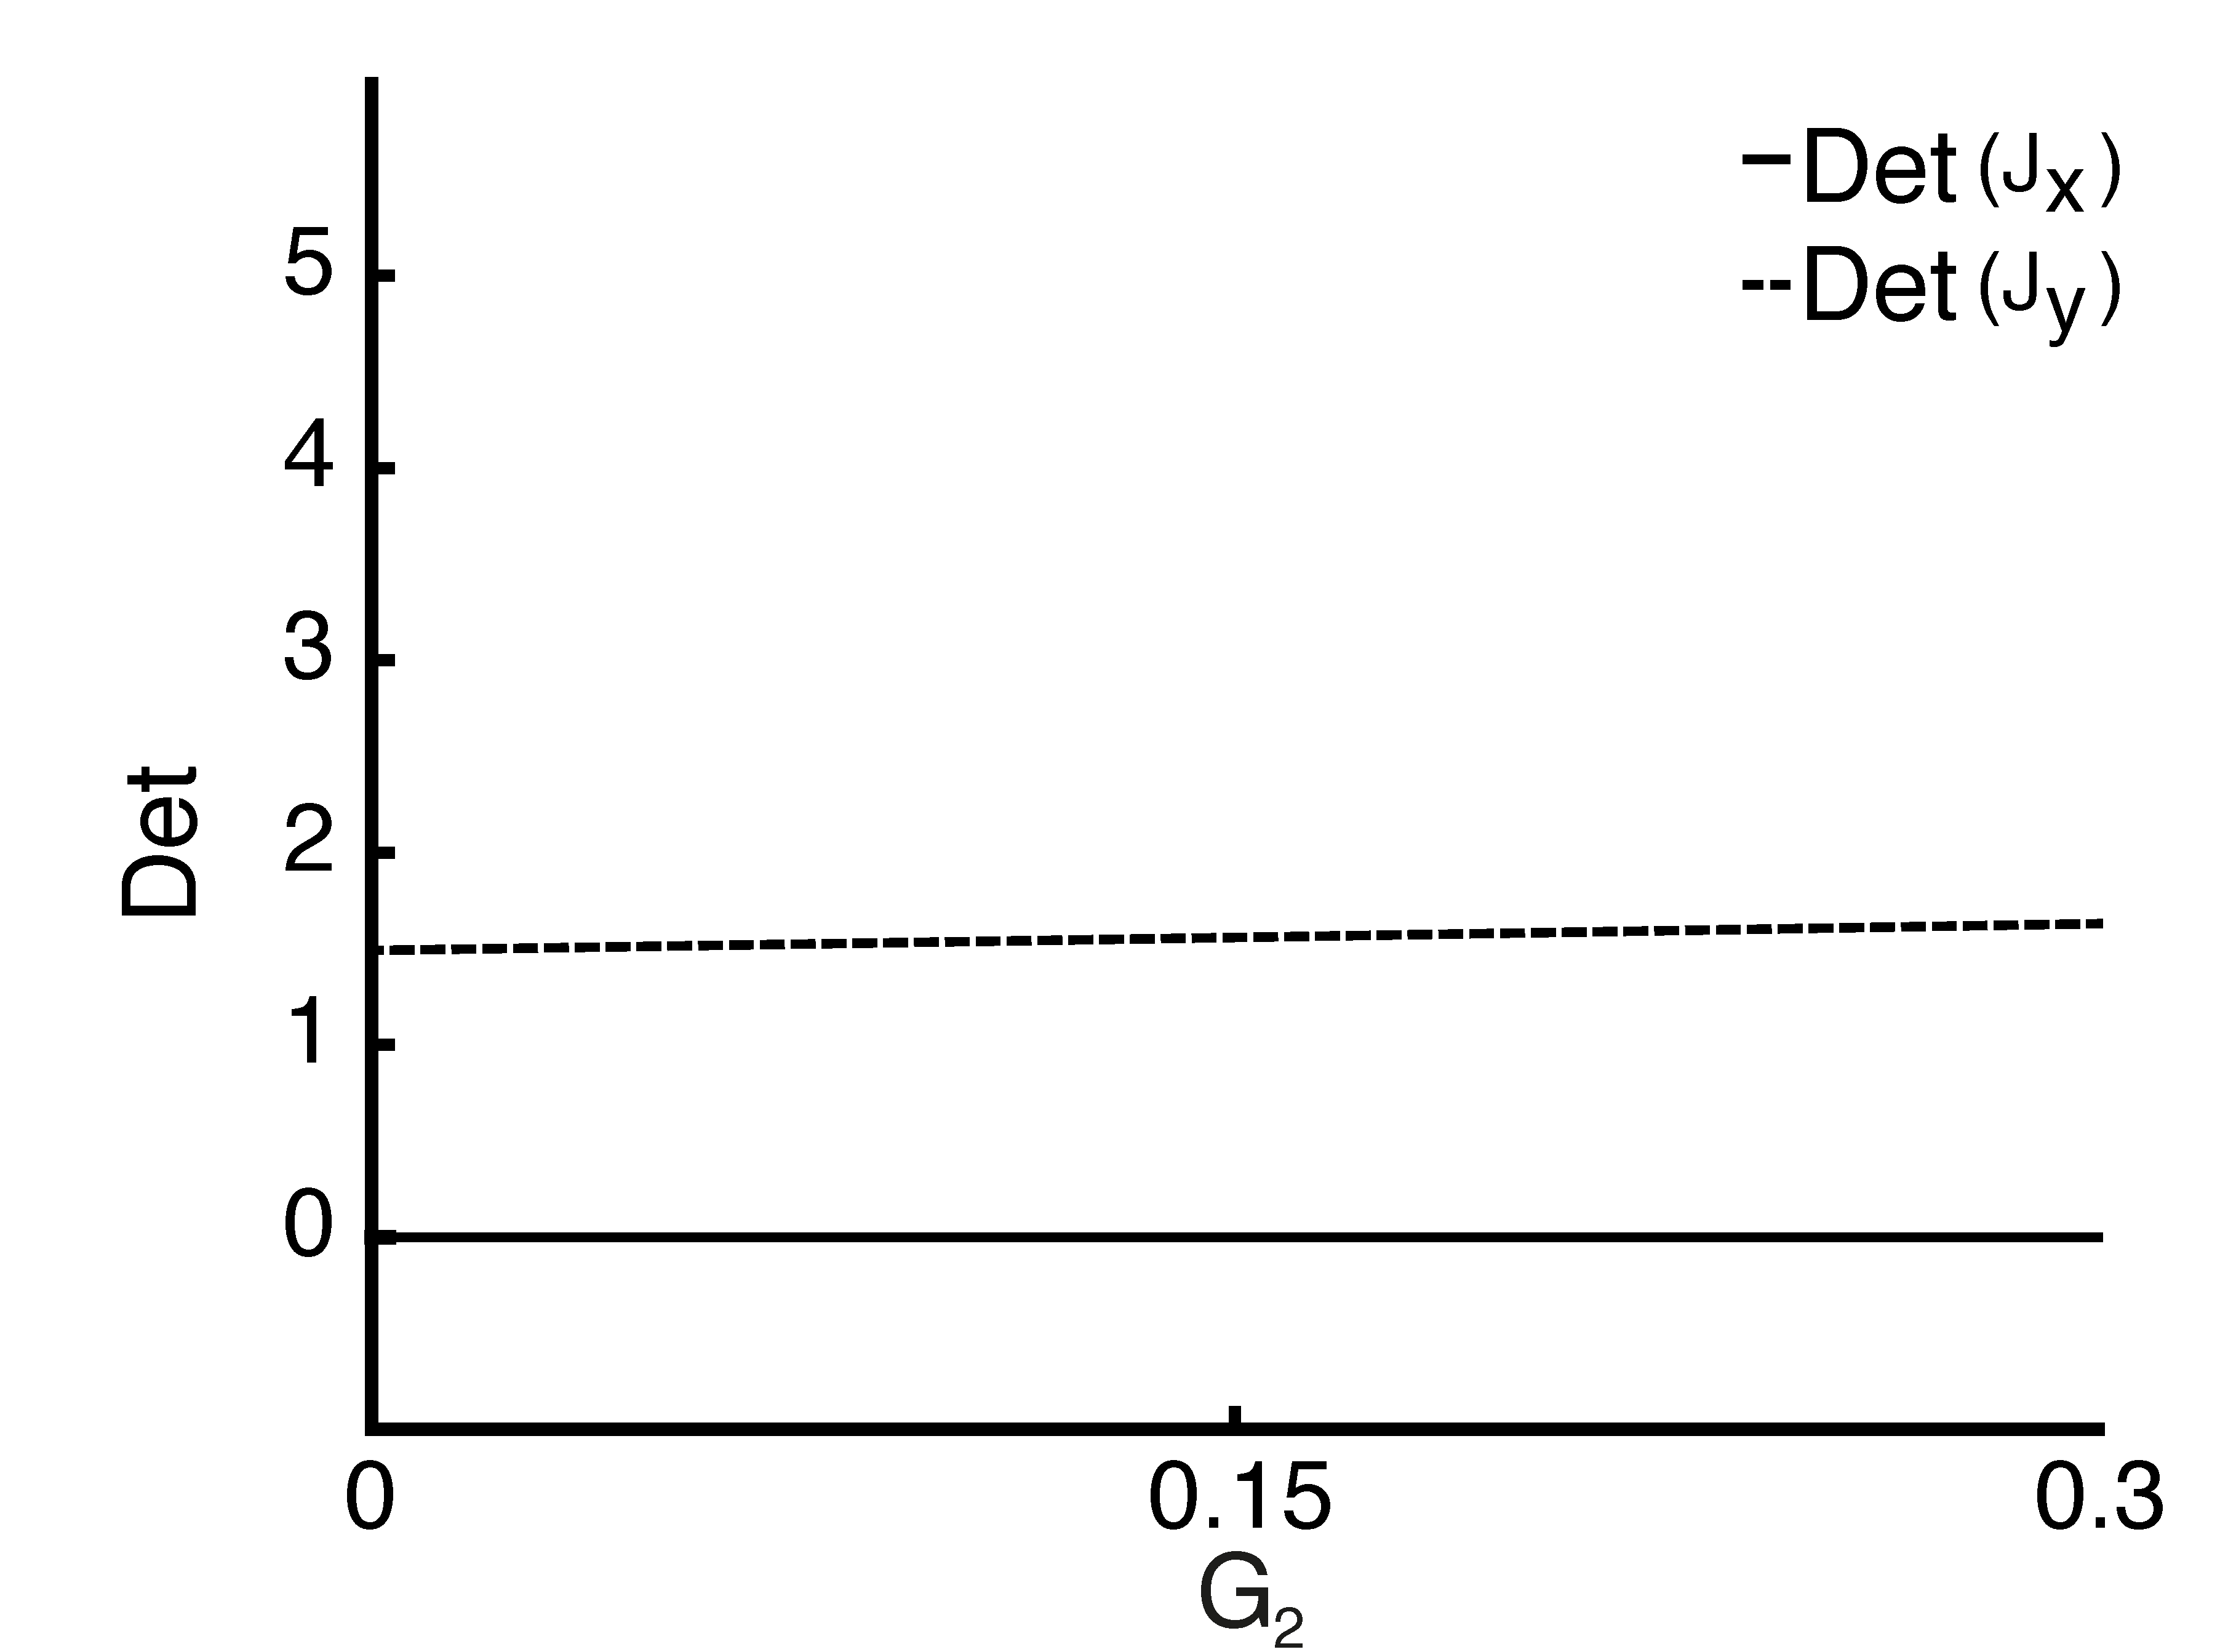
\includegraphics[width=\linewidth]{Figure4.pdf}
               \label{fig:}
       \end{subfigure}
  		 \begin{subfigure}{0.49\textwidth}
               \caption{\hspace*{\fill}}
               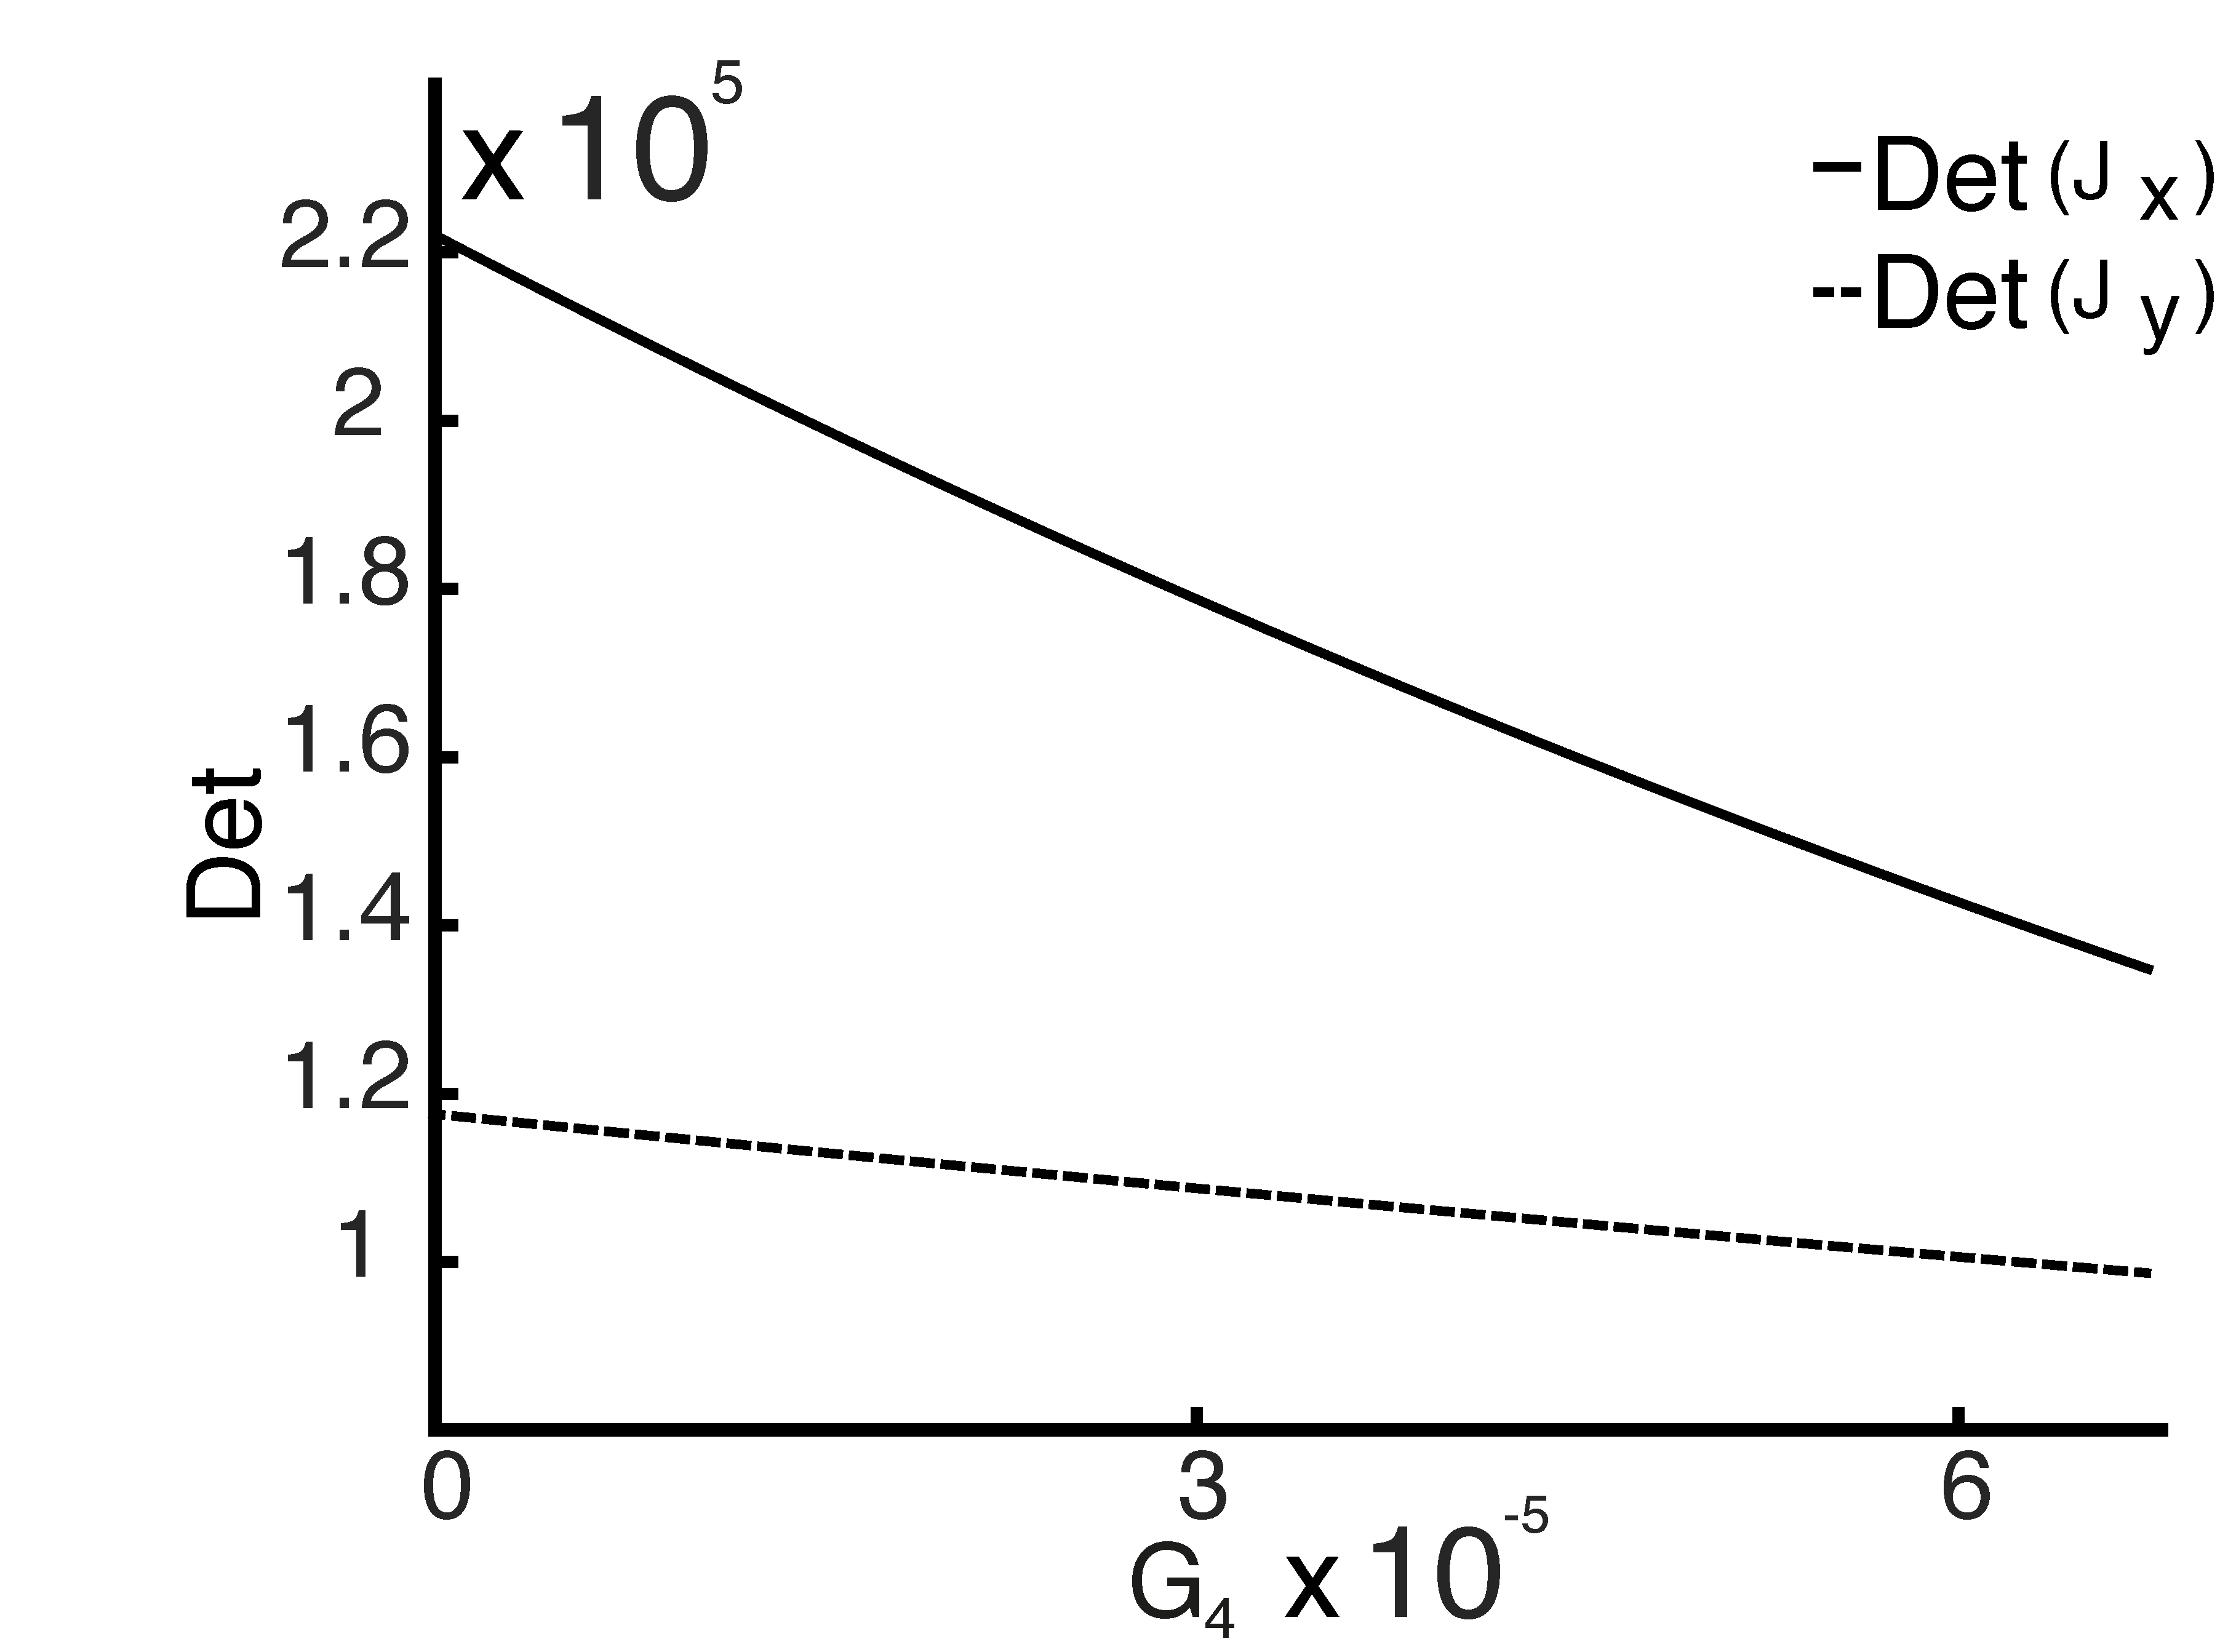
\includegraphics[width=\linewidth]{Figure5.pdf}
               \label{fig:}
       \end{subfigure}                
       \caption{The effect the density/activity parameters $G_2$ and $G_4$ have on the secretion model. \textbf{A}. When the parameter $G_4$ is varied from its maximum of 6.74$e{-5}$ to 0, depicted by the bold line, the fluid flow rate $Q$ decreases up to approximately 25$\%$. In contrast, when the parameter $G_2$=0 (depicted by the dashed line), $Q$ decreases by a negligible amount. \textbf{B}. Impact of the reaction rate parameter $\lambda_{11}$ of the Ae4 flux term has in eq.~\eqref{eq:non_Q}. A small change in the parameter causes a big variation in the total fluid flow rate of the secretion model. This result supports claims that the co-trasnport of $\na$ by the Ae4 is the responsible for the decrease in the model's salivary ouput (upon knockout), observed in \cite{siguenza2017Ae4}. \textbf{C}. Non-dimensional ionic variables $x$, $y$, $z$ as a function of the density parameter $G_2$. As the density $G_2$ approaches zero, $x$, $y$, and $z$ vary less than $1\%$. \textbf{D}. Non-dimensional ionic variables $x$, $y$, $z$ normalised as a function of the density parameter $G_4$. As $G_4$ approaches zero is of around $15\%$, whereas the variation in $y$ is approximately 6$\%$. \textbf{E}. Variation, from 0.347 to 0, in the density parameter $G_2$ has minimal effect on Det$(J_x)$ and Det$(J_y)$. The rate of change, minimal, explains why simulations of Ae2 knockout in \cite{siguenza2017Ae4} produce no changes in the total fluid flow rate of the secretion model. \textbf{F}. Variation, from 6.74$e{-5}$ to 0, in the density parameter $G_4$ has a relatively big effect on Det$(J_x)$ and Det$(J_y)$. The rate of change of Det($J_x$) reflects the system's dependence on the rate at which $\na$ bings and its extruded from the cell by the Ae4 exchanger. This is given by the parameter $\lambda_{11}$ (see Table~\ref{table:lambda}).}
       \label{fig:Continuation}      
\end{figure}
%%%%%%%%%%%%%%%%%%%%%%%%%%%

We begin our analysis by computing the flow rate equation (eq.~\ref{eq:non_Q}) as a function of the density/activity parameters $G_2$ and $G_4$ (or $Q = Q(G_i)$, where $i=2$ or $4$). The parameter $G_2$ is varied from its maximum value of 0.347 to 0, whereas $G_4$ is similarly reduced from its maximum value of 6.74$e{-5}$ to 0. As these parameters represent exchanger densities, in doing so, we are effectively reproducing the knockout simulations in \cite{siguenza2017Ae4}. In Fig.~\ref{fig:Continuation} \textbf{A} it is possible to see that as $G_2$ approaches zero, the flow rate $Q(G_2)$ is negligibly reduced from its original value (normalised to 1 when $G_2=0.347$). In contrast, as $G_4$ approaches zero, $Q(G_4)$ loses approximately 25$\%$ of its original value.\\

In their study \cite{siguenza2017Ae4} mention that it is an increase in intracellular $\na$, a consequence of loosing the Ae4 whose $\cl$/$\hco$ exchange is supported by the cation, the responsible for the observed decrease in fluid flow rate. In Fig.~\ref{fig:Continuation} \textbf{C} $\&$ \textbf{D} we explore the effect of $x(G_i)$, $y(G_i)$, and $z(G_i)$ as the density $G_i$ ($i = 2$ or 4, respectively) is varied from their normal value to 0.  In Fig.~\ref{fig:Continuation} \textbf{C} we see that $y$ is slightly affected by the decrease in $G_2$ (of less than $1\%$), this decrease is negligible in the total fluid flow rate (eq.~\ref{eq:non_Q}). On the other hand, Fig.~\ref{fig:Continuation} \textbf{D} depicts the variation on $x$ and $z$ as $G_4$ approaches zero is of around $15\%$, whereas the variation in $y$ is less than 1$\%$.\\

The rate at which fluid flow rate varies as $G_i$ ($i = 2$ or 4, respectively) approaches zero is important as it is linked to the parameters that dictate the rate at which ions are transported across the PM by the exchangers. Therefore, we calculate:
\begin{align}
\frac{dQ}{dG_i}=-\lambda_{21} \Bigg( \frac{dx}{dG_i} + \frac{dy}{dG_i} \Bigg),
\label{eq:dQ}
\end{align}
where $Q$ is defined by eq.~\eqref{eq:non_Q} and  $i = 2$ or 4, respectively. To compute the equation and its derivatives, we solve the following equation:
\begin{align}
\frac{d\bar{\textbf{F}}}{dG_i}=\frac{\partial \bar{\textbf{F}}}{\partial \bar{\textbf{x}}} \frac{d\bar{\textbf{x}}}{dG_i}+\frac{\partial \bar{\textbf{F}}}{\partial G_i} = \bar{\textbf{0}},
\end{align}
where, 
\begin{align*}
\frac{\partial \bar{\textbf{F}}}{\partial \bar{\textbf{x}}} = \begin{pmatrix}
\dfrac{\partial f_1}{\partial x} && \dfrac{\partial f_1}{\partial y} && \dfrac{\partial f_1}{\partial z} \\
\\
\dfrac{\partial f_2}{\partial x} && \dfrac{\partial f_2}{\partial y} && \dfrac{\partial f_2}{\partial z} \\
\\
\dfrac{\partial f_3}{\partial x} && \dfrac{\partial f_3}{\partial y} && \dfrac{\partial f_3}{\partial z}
\end{pmatrix}, \
\frac{\partial  \bar{\textbf{F}} }{\partial G_4}= 
\begin{pmatrix}
z \lambda_{12}-x \lambda_{11} \\
0\\
0
\end{pmatrix}, \ \ \text{and} \quad 
\frac{\partial  \bar{\textbf{F}} }{\partial G_2}= 
\begin{pmatrix}
0\\
0\\
\lambda_{17} - \frac{\lambda_{18}z}{\lambda_{19} + z}
\end{pmatrix}.
\end{align*}
Here, $f_1$, $f_2$, and $f_3$ are defined by eqs.~(\ref{eq:f1}-\ref{eq:f3}). And thus,
\begin{align*}
\begin{pmatrix}
\dfrac{\partial f_1}{\partial x} && \dfrac{\partial f_1}{\partial y} && \dfrac{\partial f_1}{\partial z} \\
\\
\dfrac{\partial f_2}{\partial x} && \dfrac{\partial f_2}{\partial y} && \dfrac{\partial f_2}{\partial z} \\
\\
\dfrac{\partial f_3}{\partial x} && \dfrac{\partial f_3}{\partial y} && \dfrac{\partial f_3}{\partial z}
\end{pmatrix}
\begin{pmatrix}
\dfrac{d x}{d G_i}\\ 
\\
\dfrac{d y}{d G_i} \\
\\
\dfrac{d z}{d G_i}
\end{pmatrix} =
- \frac{d\bar{\textbf{F}}}{dG_i}.
\end{align*}
The Jacobian matrix ($\frac{\partial \bar{\textbf{F}}}{\partial \bar{\textbf{x}}}$) was calculated using the software Wolfram-Mathematica, yet the results are not presented here due to space constraints. However, any basic symbolic solver should be able to handle this task. In our quest to compute eq.~\eqref{eq:dQ} we note that the solution can be computed by using Cramer's Rule, namely: 
\begin{align*}
\text{Det}(J) \Big(\frac{d x}{d G_i} \Big)=\text{Det}(J_x),\ \ \text{Det}(J) \Big( \frac{d y}{dG_i} \Big)=\text{Det}(J_y), \ \ \text{Det}(J) \Big( \frac{d z}{dG_i} \Big) =\text{Det}(J_z),
\end{align*}
where
{ \small
\begin{align*}
J_x=\begin{pmatrix}
-\dfrac{\partial f_1}{\partial G_i} && \dfrac{\partial f_1}{\partial y} && \dfrac{\partial f_1}{\partial z} \\
\\
-\dfrac{\partial f_2}{\partial G_i} && \dfrac{\partial f_2}{\partial y} && \dfrac{\partial f_2}{\partial z} \\
\\
-\dfrac{\partial f_3}{\partial G_i} && \dfrac{\partial f_3}{\partial y} && \dfrac{\partial f_3}{\partial z}
\end{pmatrix},
\ \
J_y=
\begin{pmatrix}
\dfrac{\partial f_1}{\partial x} && -\dfrac{\partial f_1}{\partial G_i} && \dfrac{\partial f_1}{\partial z} \\
\\
\dfrac{\partial f_2}{\partial x} && -\dfrac{\partial f_2}{\partial G_i} && \dfrac{\partial f_2}{\partial z} \\
\\
\dfrac{\partial f_3}{\partial x} && -\dfrac{\partial f_3}{\partial G_i} && \dfrac{\partial f_3}{\partial z}
\end{pmatrix},
\ \
J_z=
\begin{pmatrix}
\dfrac{\partial f_1}{\partial x} && \dfrac{\partial f_1}{\partial y} && - \dfrac{\partial f_1}{\partial G_i} \\
\\
\dfrac{\partial f_2}{\partial x} && \dfrac{\partial f_2}{\partial y} &&\dfrac{\partial f_2}{\partial G_i} \\
\\
\dfrac{\partial f_3}{\partial x} && \dfrac{\partial f_3}{\partial y} && -\dfrac{\partial f_3}{\partial G_i}
\end{pmatrix}.
\end{align*}
}
\clearpage
To illustrate our point we limit our analysis to the computation of Det$(J_x)$. This is because this represents the behaviour of the $\na$ ion, claimed to be responsible for the dynamics that led to the results presented in \cite{siguenza2017Ae4}. However, a numerical representation of the determinants, Det$(J_x)$ and Det$(J_y)$ (because the variables $x$ and $y$ determine the fluid flow rate $Q$) with respect to $G_2$ and $G_4$, can be found in Figs.~\ref{fig:Continuation}.~\textbf{E} $\&$ \textbf{F}.\\

And thus, computing Det$(J_x)$ with respect to $G_2$ we obtain:
\begin{align*}
\text{Det}(J_{x_2})=\Big(\dfrac{z \lambda_{18}}{z+\lambda_{19}} - \lambda_{17} \Big) \Lambda_1.
\end{align*}
%where,
%\begin{align*}
%& \beta_1=2 x^2 y^2 z^3 \Big( \lambda_2 \lambda_3 + \lambda_1 \lambda_4 \Big)^2, \\
%& \beta_2= - xyz^2 \Big(\lambda_2 \lambda_3 + \lambda_4 \Big(\lambda_1+ (2 \lambda_3 + xy z^2  \lambda_4) \lambda_{14} \Big) \Big)- \lambda_3^2 \lambda_{14}, \\
%& \beta_3=\lambda_{12} {\color{red}G_{4}} \Big(\lambda_{3}+xyz^2 \lambda_4 \Big)^2 - 2 xyz  \Big( \lambda_2 \lambda_3 + \lambda_1 \lambda_4\Big),\\
%&\beta_4=y\Big( \lambda_3 + xyz^2  \lambda_4\Big)^4.
%\end{align*}
In Fig.\ref{fig:Continuation}.~\textbf{E} a plot using the steady state solutions of the system (see Table~\ref{table:lambda}) demonstrates how the variation, from 0.347 to 0, in the density parameter {\color{red}$G_2$} has minimal effect on Det$(J_x)$ and Det$(J_y)$. Thus, the effect on the fluid flow rate equation is negligible. Mathematically, this is because $\Lambda_1$ has a magnitude of order 1 for all values of $x(G_2), y(G_2) $ and $z(G_2)$ (see Fig.\ref{fig:Continuation}~\textbf{B}). This indicates that the size of the determinant is entirely given by the expression:
\begin{align*}
\Big(\dfrac{z \lambda_{18}}{z+\lambda_{19}} - \lambda_{17} \Big). 
\end{align*}
which has a magnitude of order 1 for all values of $G_2$. So any relatively small (physiologically accepted) change in the parameters that constitute the expression have minimal effect.\\

In contrast, we see that variation in the density parameter $G_4$ has a big impact on the determinants of $J_x$ and $J_y$ (Fig.\ref{fig:Continuation}~\textbf{F}). And thus, the consequence is a big variation on the fluid flow rate equation (see eq.~\ref{eq:dQ}). Computing Det$(J_x)$ explicitly with respect to $G_4$, we obtain:
\begin{align*}
& \text{Det}(J_{x_4})=(x \lambda_{11}- z\lambda_{12}) \Lambda_2.
\end{align*}
%where,
%\begin{align*}
%&\delta_1=-6 x^2 y^2 z^2  \Big( \lambda_2 \lambda_3 + \lambda_1 \lambda_4 \Big)^2 \Big(z+\lambda_{19} \Big)^2,\\
%& \delta_2= z \Big(\lambda_3+xyz^2\lambda_4 \Big)^2 \beta_2\Big(z+\lambda_{19} \Big)^2,\\
%&\delta_3= -\dfrac{6 x y z  \Big( \lambda_2 \lambda_3 + \lambda_1 \lambda_4 \Big)}{\Big( \lambda_3+ \lambda_4 x y z^2  \Big)^2}-\dfrac{\lambda_{16}}{z} - \frac{\lambda_{18} \lambda_{19} G_2}{\Big( z+ \lambda_{19}\Big)^2},\\
%& \delta_4=yz \Big( \lambda_3+ \lambda_4 x y z^2 \Big)^4 \Big(z+\lambda_{19} \Big)^2.
%\end{align*}
%(the parameters $\lambda$ can be found in Table~\ref{table:lambda}). 
Note that $\Lambda_2$ has a magnitude of order 1 for all values of $x(G_4), y(G_4) $ and $z(G_4)$, for all values of $G_4$ $\in [0, 6.74e-5]$. However, the expression
\begin{align*}
(x \lambda_{11}- z\lambda_{12}) 
\end{align*}
has an order of magnitude $10^{4}$. As a consequence, when the density parameter $G_4$ approaches zero, it greatly affects the variables $x$ and $z$. This change is reflected on the fluid flow rate equation $Q$ (see Fig.~\ref{fig:Continuation}.~\textbf{B}).\\ 

Additionally we see that variation of the parameter $\lambda_{11}$, related to $x$, causes great variation on eq.~\eqref{eq:dQ}. In Fig.~\ref{fig:Continuation}.~\textbf{B}, variation of $\lambda_{11}$ as a function of $dQ/d{G_4}$ was performed to investigate how much of an impact the parameter has on fluid secretion. The results indicate that the value of the parameter, which represents the rate at which $\na$ binds and it is extruded by the Ae4 exchanger is critical in the model. This supports the results of \cite{siguenza2017Ae4} that indicate that the $\na$ dependence of the Ae4 is the responsible for the reduction in salivary gland fluid rate upon Ae4 knockout.\\

In summary, the reason for the behaviour of the system is the choice of parameters of the Ae4 model. However, note that such parameters were not chosen randomly, that is, they were carefully tuned to achieved an accurate physiological resting state that reflects that of the laboratory data and previous literature. The model indicates that the rate at which the $\na$ ion binds and it is extruded by the Ae4 greatly impacts the osmotic balance required for optimal gland fluid flow rate.